% !TEX root = master_thesis.tex

%==============================================================================
\chapter{Introduction}
\label{chap:intro}
%This chapter will give a brief introduction into the theoretical concepts that motivate this work. First the Standard Model of Particle Physics is sketched along with characteristics of the strong interaction. Next, the photoproduction of mesons and the importance of polarization observables is explained. Lastly the particular motivation and structure of this work will be presented.
%==============================================================================
%\section{The Standard Model of Particle Physics}
The \emph{Standard Model of Particle Physics} (SM) is the most successful model aiming to describe the particles and forces of the universe. It distinguishes between \emph{fermions} and \emph{bosons}. While all matter consists of fermions, bosons are particles that mediate the fundamental interactions.

Matter consists of (anti-)quarks and (anti-)leptons with three generations of each. Table \ref{tab:sm0} shows all elementary fermions including some of their most important properties. Only the first and lightest generation consists of stable particles, i.e. the up and down quark as well as the electron and its neutrino. All other particles are heavier and not stable, they will thus decay fast via the strong, electromagnetic or weak interaction.

There are in fact four interactions described by the SM: strong, electromagnetic, weak and gravitational interaction \footnote{they are ordered here according to their relative strength}, where gravitation is mentioned here for the sake of completeness; on the mass scale of elementary particles gravitation is negligible. Strong and weak interaction are restricted to a finite range of the order of the nucleon radius, whereas electromagnetic interaction and gravitation have infinite range. Each interaction has its own coupling (charge). The strong interaction is mediated by gluons and couples to the color charge.% A summary of the SM interactions can be found in table \ref{tab:sm1}.
\begin{table}[htbp]
	\centering
	\begin{tabular}{cccccc}
		\toprule
		&\multicolumn{3}{c}{Generation}&el. charge&color charge\\
		&1 & 2 & 3 & & \\
		\hline
		Quarks & $u$&$c$&$t$& 2/3 & r,g,b\\
		&$d$&$s$&$b$& 1/3 & r,g,b\\
		Leptons& $e$&$\mu$&$\tau$&-1& -\\
		& $\nu_e$&$\nu_\mu$&$\nu_\tau$&0&-\\
		\bottomrule

	\end{tabular}
\caption{Summary of the particles of the SM}
\label{tab:sm0}
\end{table}
%\begin{table}[htbp]
%	\centering
%	\begin{tabular}{ccc}
%		\toprule
%		interaction & couples to & Gauge boson\\
%		\hline
%		strong & color & $g$\\
%		elm.& el. charge & $\gamma$\\
%		weak&weak charge & $W^\pm,Z^0$\\
%		\bottomrule
%	\end{tabular}
%
%	\caption{Summary of the interactions of the SM}
%	\label{tab:sm1}
%\end{table}



Gluons and quarks carry color charge and thus interact strongly. However, an isolated quark or gluon has not been observed. Only color neutral bound systems of quarks are seen, which are called hadrons. Hadrons with integer spin are called mesons and those with half-integer spin are called baryons. Color neutrality demands mesons consist of at least one quark and one anti-quark and baryons consist of at least three quarks.


 As already mentioned, isolated quarks are not seen. This can be understood in terms of the strong coupling constant $\alpha_s$. The coupling constant is a measure of the strength of the strong interaction. Because it is highly dependent on the momentum transfer in the observed strong reaction it is also called running coupling constant, which is depicted in figure \ref{fig:coupl}.
 \begin{figure}
 	\centering
 	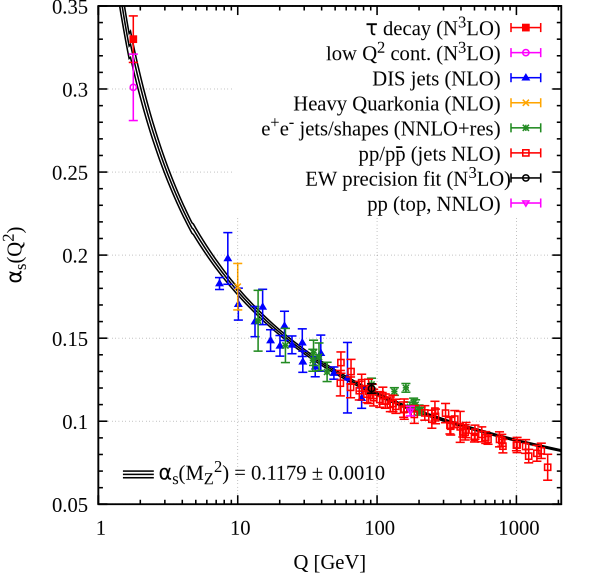
\includegraphics[width=.5\linewidth]{qcd}
 	\caption{Running coupling of QCD. The colored data points represent different methods to obtain a value for $\alpha_s$. For more details it may be referred to \cite{pdg}.}
 	\label{fig:coupl}
 \end{figure}

 For low ($<\SI{1}{\GeV}$) momentum transfers or large distances the coupling constant approaches infinity whereas it decreases for high ($\gg\SI{1}{\GeV}$) momentum transfers or short distances. These momentum ranges are referred to as \emph{confinement} and \emph{asymptotic freedom}, respectively; quarks are confined to remain in a bound state since if one tried to pull them apart the color field becomes so strong it will create a new quark anti-quark pair resulting in two new bound states. On the other hand, bound quarks behave quasi-free and can be described using perturbative quantum chromodynamics (pQCD) if probed at sufficiently large momentum transfers.

 It is more difficult however to describe QCD at momentum scales of $\approx \SI{1}{\GeV}$ since the coupling is too strong to justify a perturbative approach. Thus explicit modeling of QCD bound states is inevitable. One possibility is to describe baryons consisting of constituent quarks which are bound in a potential. Constituent quark models assume baryons are made up of three constituent quarks with effective masses differing from the bare quark mass. The effective mass is made up mostly from a sea of quark anti-quark pairs and gluons which surround the bare (valence) quarks. The explicit form of the binding potential is determined for each model.

 The Bonn model \cite{bonnmodel}, for example, is formulated as a relativistically covariant constituent quark model.
 A potential increasing linearly with the distance is employed to adequately describe confinement. The binding potential between the constituent quarks is described by an instanton-induced interaction. Baryon resonances are then states with an orbital or angular excitation of one of the quarks. Figure \ref{fig:bm} shows computed nucleon, that is Isospin $I=1/2$ resonances, of the Bonn model \cite{bonnmodel} on the left side of each column. These are compared to measured resonances and their PDG rating \cite{pdg} in the middle. Uncertainties are indicated by the colored areas. The resonances are identified by their total angular momentum and their parity $J\pi$. In addition also the total internal angular momentum along with isospin and again the total angular momentum $L_{2T2J}$ is given.
  \begin{figure}[htbp]
 	\centering
 	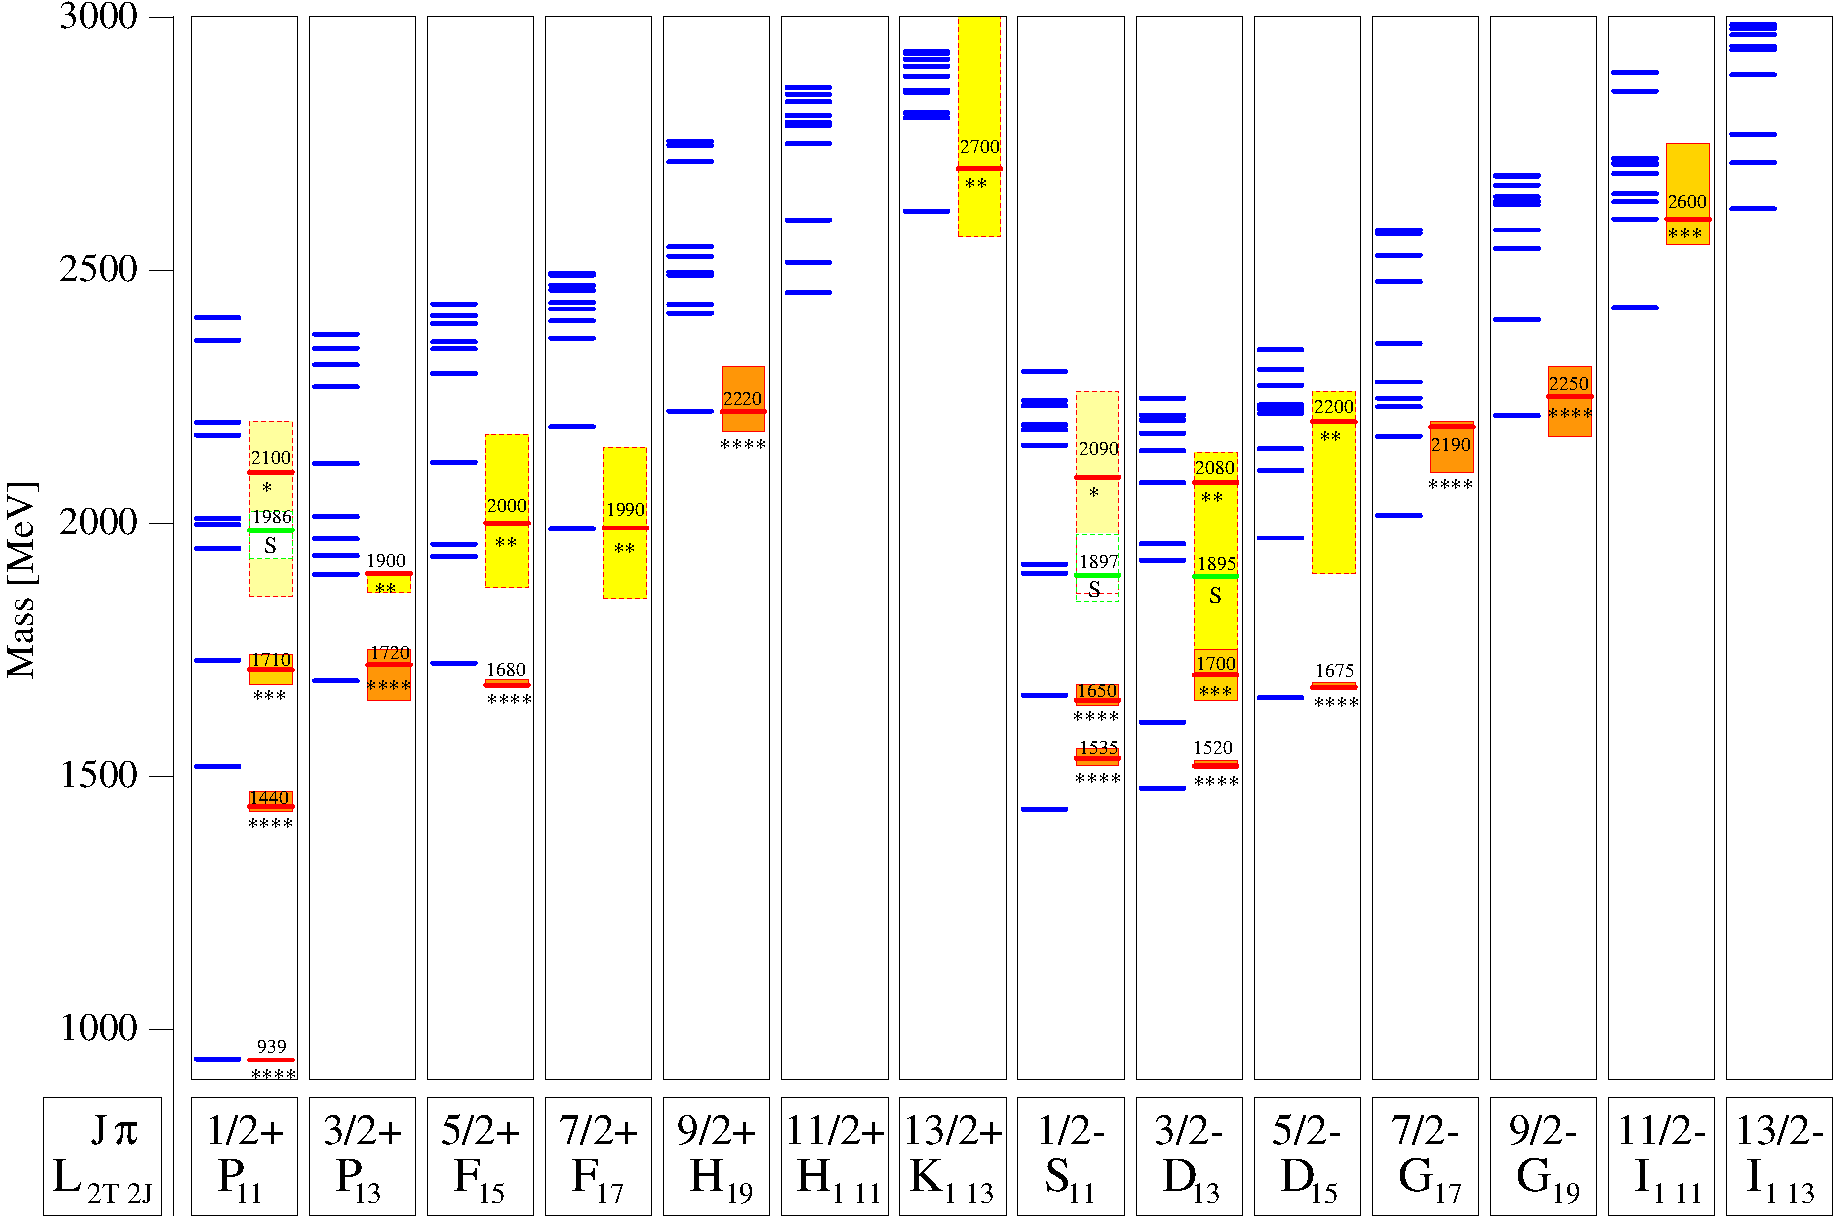
\includegraphics[width=\linewidth]{figs/NucM2.pdf}
 	\caption{Calculated nucleon (isospin $I=1/2$) resonances compared to measurements. Left in each column are the calculations \cite{bonnmodel}, the middle shows the measurements and PDG rating \cite{pdg}}
 	\label{fig:bm}
 \end{figure}
While generally good agreement exists for low lying resonances, especially for high masses there are much more resonances predicted than actually found. This is also known as the problem of the \enquote{missing resonances} indicating the poor understanding of QCD in the non-perturbative region. This can be due to several reasons: most of the knowledge about nucleon resonances and their properties was obtained investigating the $\pi N$ channel, biasing the data for resonances coupling weakly to this channel. Furthermore, the number of excited states with definite quantum numbers is related directly to the effective number of degrees-of-freedom accessible to the underlying theory. As a consequence, the number of degrees-of-freedom should be obtainable by comparing the measured states to the predicted states. Since nucleon resonances decay dominantly hadronic, their resonances are broad and overlapping. Thus on one hand the determination of excitation spectra proves to be a challenge on its own, demanding sophisticated methods, such as partial wave analysis (PWA). On the other hand it is not yet clear how many effective degrees-of-freedom exist for the nucleon in a constituent quark model. They could for example be decreased if the nucleon were made up of a quark and a di-quark structure. In either case it should prove fruitful to investigate the photoproduction of mesons off the nucleon for different final states to access the resonances and transitions between them which are of interest. This should ultimately add to the understanding of QCD in the non-perturbative regime. \cite{Krusche}


\section{Photoproduction of Pseudoscalar Mesons}
From the scattering theory point of view, photoproduction of mesons is well understood \cite{Krusche}. Figure \ref{fig:mes_bildchen} shows schematically the process thereof off the proton:

\begin{figure}[htbp]
	\centering
	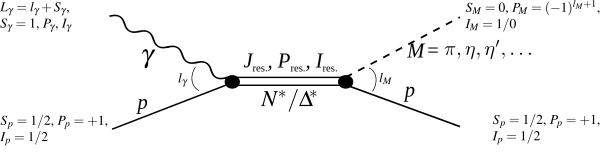
\includegraphics[width=\linewidth]{meson_bildchen}
	\caption{\textsc{Feynman} diagram for the s-channel photoproduction of pseudoscalar mesons, adapted from \cite{farahphd}}
	\label{fig:mes_bildchen}
\end{figure}

The analysis requires partial wave decomposition in both initial and final states \cite{Drechsel} since the intermediate resonance has definite angular momentum, parity  and isospin $J_\text{res.}, P_\text{res.}, I_\text{res.}$. The resonance is excited by a photon with (iso-) spin $I_\gamma,S_\gamma =1$ and parity $P_\gamma$ coupling electromagnetically to the target proton with (iso-) spin $I_p=1/2,S_p=1/2$ and parity $P_p$. The relative momentum is $l_\gamma$, such that the total momentum of the photon is $L_\gamma=l_\gamma+S_\gamma$. Subsequently the intermediate state will have the quantum numbers $J_\text{res.}, P_\text{res.}, I_\text{res.}$ and decay into a pseudoscalar ($S_M=0$) meson with isospin $I_M$, relative orbital angular momentum $l_M$ und Parity $P_M=(-1)^{l_M+1}$ and a proton. The following selection rules can be derived using parity and momentum conservation \cite{Krusche,farahphd}
\begin{align}
	%\left|L_\gamma-S_p\right|&=\left|L_\gamma-1/2\right|\leq J_\text{res.}\leq\left|L_\gamma+1/2\right|=\left|L_\gamma+S_p\right|,\\
	J_\text{res.}&=L_\gamma\oplus S_p = L_\gamma\oplus 1/2,\\
	P_\text{res.}&=P_p\cdot P_\gamma=P_\gamma,\\
	%\left|l_M-S_p\right|&=\left|l_M-1/2\right|\leq J_\text{res.}\leq\left|l_M+1/2\right|=\left|l_M+S_p\right|,\\
	J_\text{res.}&=l_M\oplus S_p = l_M\oplus 1/2\\
	P_\text{res.}&=P_p\cdot P_M=(-1)^{l_M+1},
\end{align}
where the usual rules for the coupling of angular momenta \cite{theo3} apply. Thus, knowledge of the photoproduction multipoles allows the identification of contributing resonances for particular mesonic final states. Table \ref{tab:qn} shows relevant resonances for the lowest order of photon multipoles ($L_\gamma=1$).

\begin{table}[htbp]
	\begin{tabular}{cccccc}
		\toprule
		E
	\end{tabular}
\caption{Allowed quantum numbers for the intermediate resonance state $N^*/\Delta^*$}
\label{tab:qn}
\end{table}

\section{Measurement of Polarization Observables}

\section{Introduction to \textsc{Bayesian} statistics}
\subsection{}

\section{Motivation and Structure of this Thesis}
bla
